\chapter{Spectral Representation and the Density of States}
\label{ch:band-to-density-of-states}

A one-electron Hamiltonian determines its available states through its spectral
representation.  The density of states is the spectral multiplicity per energy
and per physical size.  For a periodic crystal, Bloch's theorem resolves the
spectrum into bands $E_n(\bm k)$, and reciprocal-space integration converts
those bands into an energy density.  Statistical mechanics enters in the next
chapter to determine occupation.

The spectral and state-counting development follows Kittel and the semiconductor
treatments of Sze and Lee, Sze and Ng, and Rudan
\cite{kittel2005,szeLee2012,szeNg2007,rudan2015}.  The analytic representation
also defines the quantities evaluated numerically later in the chapter.

\section{Spectral representation and discrete multiplicity}

Let the finite one-electron Hamiltonian $\hat H$ have distinct eigenvalues
$E_j$.  An orthonormal basis for the eigenspace at $E_j$ is
\begin{equation}
  \{\ket{j,a}:a=1,\ldots,M_j\},
  \label{eq:energy-eigenspace-basis}
\end{equation}
where $M_j$ is the multiplicity of that eigenvalue.  The projector onto the
complete eigenspace is
\begin{equation}
  \hat P_j
  =\sum_{a=1}^{M_j}\ket{j,a}\bra{j,a}.
  \label{eq:energy-eigenspace-projector}
\end{equation}
Its trace equals the multiplicity:
\begin{equation}
  M_j=\dim\operatorname{Ran}\hat P_j
  =\operatorname{Tr}\hat P_j.
  \label{eq:discrete-energy-multiplicity}
\end{equation}
The spectral representations of the Hamiltonian and identity are
\begin{equation}
  \boxed{
  \hat H=\sum_jE_j\hat P_j,
  \qquad
  \hat I=\sum_j\hat P_j.
  }
  \label{eq:hamiltonian-spectral-representation}
\end{equation}

A function of the Hamiltonian acts on each eigenspace through its eigenvalue:
\begin{equation}
  F(\hat H)=\sum_jF(E_j)\hat P_j.
  \label{eq:function-of-hamiltonian-spectral-representation}
\end{equation}
For the spectral delta distribution,
\begin{equation}
  \delta(E-\hat H)
  =\sum_j\delta(E-E_j)\hat P_j.
  \label{eq:spectral-delta-operator}
\end{equation}
Taking the trace gives the discrete density of states:
\begin{equation}
  \boxed{
  G(E)
  =\operatorname{Tr}\delta(E-\hat H)
  =\sum_jM_j\delta(E-E_j).
  }
  \label{eq:discrete-density-of-states-distribution}
\end{equation}
This trace is basis independent.  It counts the full eigenspace at each energy
and is determined by the spectrum of $\hat H$.
Integrating across an interval counts the states inside it:
\begin{equation}
  \int_{E_a}^{E_b}G(E)\,\dd E
  =\#\{\alpha:E_a\le E_\alpha\le E_b\},
  \label{eq:discrete-dos-interval-count}
\end{equation}
with the usual endpoint convention understood.

A finite energy measurement has a resolution $\Delta E$.  If energy bin $b$
contains $M_b$ states, the state density in that bin is
\begin{equation}
  g(E_b)
  \simeq\frac{M_b}{\mathcal V_d\,\Delta E},
  \label{eq:dos-from-discrete-bin-multiplicity}
\end{equation}
where $\mathcal V_d$ is the system's length, area, or volume in $d$ dimensions.
As the physical system becomes large, neighboring levels become closely spaced.
The discrete multiplicities within narrow energy intervals then approach a
smooth density:
\begin{equation}
  \boxed{
  g(E)
  =\lim_{\Delta E\to0}
   \frac{M(E,E+\Delta E)}{\mathcal V_d\,\Delta E}.
  }
  \label{eq:dos-continuum-limit-of-multiplicity}
\end{equation}
The limit is understood together with the thermodynamic limit: the physical
system grows so that every small but finite energy interval contains enough
closely spaced states to define a density.

The cumulative or integrated density of states is the trace of the spectral
projector below $E$:
\begin{equation}
  \mathcal N(E)
  =\frac{1}{\mathcal V_d}
   \operatorname{Tr}\Theta(E-\hat H)
  =\frac{1}{\mathcal V_d}
   \sum_jM_j\Theta(E-E_j).
  \label{eq:discrete-integrated-density-of-states}
\end{equation}
It is a staircase for a finite system.  The height of each step is the
multiplicity of the corresponding energy, divided by physical size.  In the
continuum limit the steps become dense and
\begin{equation}
  g(E)=\frac{\dd\mathcal N}{\dd E}.
  \label{eq:dos-derivative-of-integrated-count}
\end{equation}
This discrete-to-continuous construction is the meaning of ``density'' in
density of states.

\begin{definition}{Density of states}{band-derived-density-of-states}
For a system of physical size $\mathcal V_d$ in $d$ spatial dimensions, the
density of states $g(E)$ is defined so that
\begin{equation}
  g(E)\,\dd E
  \label{eq:dos-operational-definition}
\end{equation}
is the number of one-particle states per $\mathcal V_d$ with energies in
$[E,E+\dd E]$.  Thus $g(E)$ is the continuum form of discrete level
multiplicity and describes state availability.
\end{definition}

\section{Bloch-band information and state density}

For a periodic effective one-electron Hamiltonian, Bloch's theorem gives
\begin{equation}
  \psi_{n\bm k}(\bm r)
  =e^{i\bm k\cdot\bm r}u_{n\bm k}(\bm r),
  \qquad
  u_{n\bm k}(\bm r+\bm R)=u_{n\bm k}(\bm r),
  \label{eq:dos-bloch-state}
\end{equation}
and the Bloch eigenvalue problem gives
\begin{equation}
  H(\bm k)u_{n\bm k}=E_n(\bm k)u_{n\bm k}.
  \label{eq:dos-bloch-eigenvalue-problem}
\end{equation}
For a finite periodic crystal, the spectral representation is
\begin{equation}
  \hat H
  =\sum_{n,\bm k}E_n(\bm k)
   \ket{n,\bm k}\bra{n,\bm k},
  \label{eq:bloch-hamiltonian-spectral-representation}
\end{equation}
with an additional sum or degeneracy factor for spin.  Its spectral trace is
\begin{equation}
  G(E)
  =g_s\sum_{n,\bm k}
   \delta[E-E_n(\bm k)].
  \label{eq:finite-bloch-spectral-density}
\end{equation}
The general object used to calculate the DOS is the resulting Bloch band
$E_n(\bm k)$.  Plane-wave, tight-binding, $\bm k\cdot\bm p$, and first-principles
Hamiltonians are different models for calculating that Bloch band.  The
nearest-neighbor tight-binding band introduced later is an exactly solvable
Bloch-band example.

A band dispersion is a function
\begin{equation}
  E_n:\bm k\longmapsto E_n(\bm k),
  \label{eq:band-as-energy-map}
\end{equation}
where $n$ labels the band and $\bm k$ lies in the first Brillouin zone.  A graph
of $E_n(\bm k)$ shows how energy changes with Bloch wave vector.  The density of
states supplies the corresponding state count on the energy axis.  Two portions
of a band can span the same energy interval while contributing very different
numbers of states.

The distinction becomes visible in one dimension.  Suppose neighboring allowed
wave vectors are separated by $\Delta k$.  If a band is steep, successive
states differ substantially in energy:
\begin{equation}
  \Delta E\simeq\left|\frac{\dd E}{\dd k}\right|\Delta k.
  \label{eq:energy-spacing-from-band-slope}
\end{equation}
The number of states per energy interval is consequently proportional to
\begin{equation}
  \frac{\Delta k}{\Delta E}
  \simeq\frac{1}{|\dd E/\dd k|}.
  \label{eq:one-dimensional-dos-slope-idea}
\end{equation}
A flat band has many nearby wave vectors within a small energy interval and
therefore a large density of states.  A steep band has a smaller density of
states.

For bulk material, $\mathcal V_3$ is a volume and $g(E)$ commonly has units
\si{\per\electronvolt\per\cubic\centi\metre}.  In a two-dimensional sheet it
is quoted per area, and in a one-dimensional channel it is quoted per length.
A density of states ``per primitive cell'' converts to a volumetric density
through the primitive-cell volume before combination with concentrations per
cubic centimetre.

\section{Allowed wave vectors in a finite periodic crystal}

Begin with a one-dimensional crystal of length $L=N_a a$, where $a$ is the
lattice period and $N_a$ is the number of primitive cells.  Impose periodic
boundary conditions on a Bloch factor:
\begin{equation}
  e^{ik(x+L)}=e^{ikx}.
  \label{eq:dos-periodic-boundary-condition}
\end{equation}
Cancelling $e^{ikx}$ gives
\begin{equation}
  e^{ikL}=1,
  \label{eq:dos-periodic-phase-condition}
\end{equation}
which requires
\begin{equation}
  k_m=\frac{2\pi m}{L},
  \qquad m\in\mathbb Z.
  \label{eq:dos-allowed-one-dimensional-k}
\end{equation}
Neighboring values are separated by
\begin{equation}
  \Delta k=\frac{2\pi}{L}.
  \label{eq:dos-one-dimensional-k-spacing}
\end{equation}
Consequently, the number of allowed $k$ values per interval $\dd k$ is
\begin{equation}
  \dd N_k=\frac{L}{2\pi}\,\dd k.
  \label{eq:dos-one-dimensional-k-count}
\end{equation}
Including a spin degeneracy $g_s$ multiplies this count by $g_s$.

For a periodic rectangular crystal with
$V=L_xL_yL_z$, the allowed vectors are
\begin{equation}
  k_i=\frac{2\pi m_i}{L_i},
  \qquad i\in\{x,y,z\},
  \label{eq:dos-three-dimensional-k-grid}
\end{equation}
and one allowed $\bm k$ point occupies reciprocal-space volume
\begin{equation}
  \Delta^3k
  =\Delta k_x\Delta k_y\Delta k_z
  =\frac{(2\pi)^3}{V}.
  \label{eq:dos-reciprocal-cell-volume}
\end{equation}
Thus
\begin{equation}
  \dd N_k
  =g_s\frac{V}{(2\pi)^3}\,\dd^3k.
  \label{eq:dos-three-dimensional-state-count}
\end{equation}
The artificial finite crystal makes the allowed states discrete.  In the
thermodynamic limit, $L_i\rightarrow\infty$, the spacings $\Delta k_i$ approach
zero and the sum over allowed vectors becomes an integral.  The state-counting
factor $V/(2\pi)^3$ remains.

\begin{modelcheck}
The first Brillouin zone contains one allowed $\bm k$ point per primitive cell
for each band, before spin is counted.  Therefore one nondegenerate band
integrated over the complete Brillouin zone contains one state per primitive
cell; with ordinary spin degeneracy it contains two.  This provides a global
normalization check for every calculated density of states.
\end{modelcheck}

\section{The general density of states of a band}

The Dirac delta distribution provides a concise way to select the wave vectors
whose energy equals $E$.  For bands $E_n(\bm k)$, the density of states per unit
volume is
\begin{equation}
  \boxed{
  g(E)
  =\frac{g_s}{(2\pi)^3}
   \sum_n\int_{\mathrm{BZ}}
   \delta\!\left[E-E_n(\bm k)\right] \,\dd^3k.
  }
  \label{eq:general-band-density-of-states}
\end{equation}
The integral is over the first Brillouin zone.  The band sum is included because
different bands can contribute states at the same energy.

To verify the meaning of this expression, integrate it over an energy interval
$[E_1,E_2]$:
\begin{equation}
\begin{aligned}
  \int_{E_1}^{E_2}g(E)\,\dd E
  ={}&\frac{g_s}{(2\pi)^3}\sum_n
  \int_{\mathrm{BZ}}\dd^3k
  \int_{E_1}^{E_2}\dd E\,
  \delta\!\left[E-E_n(\bm k)\right].
\end{aligned}
  \label{eq:dos-energy-window-derivation}
\end{equation}
The inner integral is one if $E_n(\bm k)$ lies inside the interval and zero
otherwise.  Equation~\eqref{eq:dos-energy-window-derivation} therefore counts
exactly the reciprocal-space states in that energy window.

\section{Constant-energy surfaces and band velocity}

For a regular energy value, the set
\begin{equation}
  S_n(E)=\{\bm k:E_n(\bm k)=E\}
  \label{eq:constant-energy-surface-definition}
\end{equation}
is a surface in reciprocal space.  The multidimensional delta-function identity
converts the Brillouin-zone integral into a surface integral:
\begin{equation}
  \boxed{
  g(E)
  =\frac{g_s}{(2\pi)^3}
   \sum_n\int_{S_n(E)}
   \frac{\dd S}{|\nabla_{\bm k}E_n(\bm k)|}.
  }
  \label{eq:dos-constant-energy-surface}
\end{equation}
This equation combines the area $\dd S$ of the constant-energy surface with the
inverse rate $1/|\nabla_{\bm k}E_n|$ at which energy changes normal to that
surface.
The semiclassical group velocity is
\begin{equation}
  \bm v_n(\bm k)
  =\frac{1}{\hbar}\nabla_{\bm k}E_n(\bm k).
  \label{eq:dos-band-group-velocity}
\end{equation}
Consequently, slowly varying portions of a band contribute strongly to the
density of states.  At a critical point where
$\nabla_{\bm k}E_n=0$, the surface formula signals a nonanalytic feature called
a van Hove singularity.  Its detailed form depends on dimensionality and on
whether the critical point is a minimum, maximum, or saddle point.

\section{Exact example: a one-dimensional tight-binding band}

Consider one orbital per primitive cell with nearest-neighbor hopping $t>0$:
\begin{equation}
  E(k)=E_0-2t\cos(ka),
  \qquad -\frac{\pi}{a}\le k<\frac{\pi}{a}.
  \label{eq:tight-binding-one-dimensional-band}
\end{equation}
The allowed energies occupy the finite interval
\begin{equation}
  E_0-2t\le E\le E_0+2t.
  \label{eq:tight-binding-band-range}
\end{equation}
Differentiate the dispersion:
\begin{equation}
  \frac{\dd E}{\dd k}=2ta\sin(ka).
  \label{eq:tight-binding-band-derivative}
\end{equation}
For an energy strictly inside the band, there are two wave-vector roots with
equal derivative magnitude.  The one-dimensional delta-function identity
\begin{equation}
  \delta[E-E(k)]
  =\sum_{k_i:E(k_i)=E}
   \frac{\delta(k-k_i)}{|\dd E/\dd k|_{k_i}}
  \label{eq:one-dimensional-delta-root-identity}
\end{equation}
gives, per primitive cell,
\begin{equation}
  g(E)
  =\frac{g_s}{2\pi}
   \sum_{k_i}\frac{a}{|\dd E/\dd k|_{k_i}}.
  \label{eq:tight-binding-dos-root-sum}
\end{equation}
From
\begin{equation}
  \cos(ka)=\frac{E_0-E}{2t},
  \label{eq:tight-binding-cosine-energy}
\end{equation}
it follows that
\begin{equation}
  |\sin(ka)|
  =\sqrt{1-\left(\frac{E-E_0}{2t}\right)^2}.
  \label{eq:tight-binding-sine-energy}
\end{equation}
Substitution of the two roots gives
\begin{equation}
  \boxed{
  g(E)
  =\frac{g_s}
   {\pi\sqrt{4t^2-(E-E_0)^2}},
  \qquad |E-E_0|<2t.
  }
  \label{eq:tight-binding-one-dimensional-dos}
\end{equation}
The density of states diverges at both band edges because the band slope
vanishes there.  The divergence is integrable: the total number of states is
finite,
\begin{equation}
  \int_{E_0-2t}^{E_0+2t}g(E)\,\dd E=g_s.
  \label{eq:tight-binding-dos-normalization}
\end{equation}

\begin{figure}[H]
  \centering
  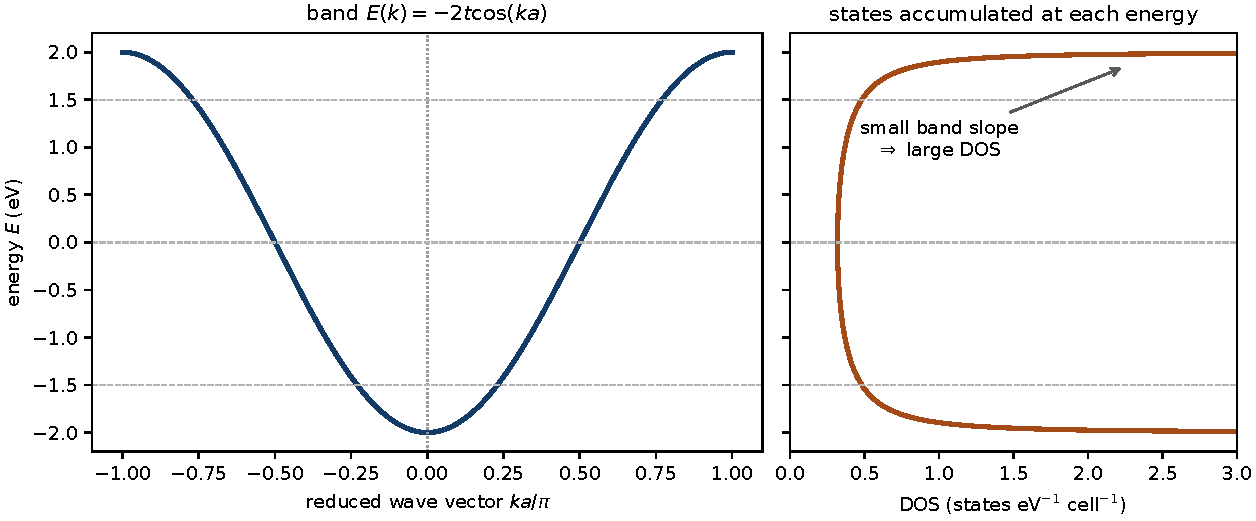
\includegraphics[width=0.90\textwidth]{figures/dos-band-to-density.pdf}
  \caption{The same one-dimensional tight-binding band shown as a dispersion
  and as a density of states.  Near a band edge, many neighboring $k$ states
  occupy a narrow energy interval because $|\dd E/\dd k|$ is small.\figurenotebookmark}
  \label{fig:dos-band-to-density}
\end{figure}
\figurenotebooktext{figures/03_spectral-density-of-states/fig_03_01.ipynb}

\section{Parabolic bands in one, two, and three dimensions}

Near a nondegenerate isotropic minimum, approximate the band by
\begin{equation}
  E(\bm k)=E_0+\frac{\hbar^2k^2}{2m^*}.
  \label{eq:dos-isotropic-parabolic-band}
\end{equation}
Define the excess energy
\begin{equation}
  \varepsilon=E-E_0\ge0.
  \label{eq:dos-parabolic-excess-energy}
\end{equation}
The constant-energy radius is
\begin{equation}
  k(\varepsilon)=\frac{\sqrt{2m^*\varepsilon}}{\hbar}.
  \label{eq:dos-parabolic-k-radius}
\end{equation}

In $d$ dimensions, the volume of a radius-$k$ ball is
\begin{equation}
  \Omega_d(k)
  =\frac{\pi^{d/2}}{\Gamma(d/2+1)}k^d.
  \label{eq:d-dimensional-ball-volume}
\end{equation}
The number of states per physical $d$-dimensional measure below energy
$E_0+\varepsilon$ is therefore
\begin{equation}
  \frac{\mathcal N_d(\varepsilon)}{\mathcal V_d}
  =\frac{g}{(2\pi)^d}
   \frac{\pi^{d/2}}{\Gamma(d/2+1)}
   \left(\frac{2m^*\varepsilon}{\hbar^2}\right)^{d/2},
  \label{eq:integrated-parabolic-state-count-d-dimensions}
\end{equation}
where $g$ contains the declared spin, valley, and band degeneracies.
Differentiating with respect to energy gives
\begin{equation}
  g_d(E)\propto(E-E_0)^{d/2-1}\Theta(E-E_0).
  \label{eq:dos-dimensional-power-law}
\end{equation}
Dimensionality determines the band-edge power law.

\subsection{One dimension}

For $d=1$,
\begin{equation}
  \boxed{
  g_{1\mathrm D}(E)
  =\frac{g}{\pi\hbar}
   \sqrt{\frac{m^*}{2(E-E_0)}}
   \Theta(E-E_0).
  }
  \label{eq:one-dimensional-parabolic-dos}
\end{equation}
The inverse-square-root edge divergence is the parabolic version of the
one-dimensional van Hove singularity.

\subsection{Two dimensions}

For $d=2$,
\begin{equation}
  \boxed{
  g_{2\mathrm D}(E)
  =\frac{g m^*}{2\pi\hbar^2}\Theta(E-E_0).
  }
  \label{eq:two-dimensional-parabolic-dos}
\end{equation}
Each ideal two-dimensional parabolic subband contributes a constant step.
Quantum wells consequently exhibit a staircase-like density of states when
several confinement subbands are included.

\subsection{Three dimensions}

For $d=3$,
\begin{equation}
  \boxed{
  g_{3\mathrm D}(E)
  =\frac{g}{4\pi^2}
   \left(\frac{2m^*}{\hbar^2}\right)^{3/2}
   \sqrt{E-E_0}\,\Theta(E-E_0).
  }
  \label{eq:three-dimensional-parabolic-dos-general-degeneracy}
\end{equation}
For spin degeneracy $g_s=2$ and no additional valley degeneracy, this becomes
\begin{equation}
  g_{3\mathrm D}(E)
  =\frac{1}{2\pi^2}
   \left(\frac{2m^*}{\hbar^2}\right)^{3/2}
   \sqrt{E-E_0}\,\Theta(E-E_0).
  \label{eq:three-dimensional-parabolic-dos-spin-two}
\end{equation}
This is the square-root form used for bulk conduction and valence bands.

\begin{figure}[H]
  \centering
  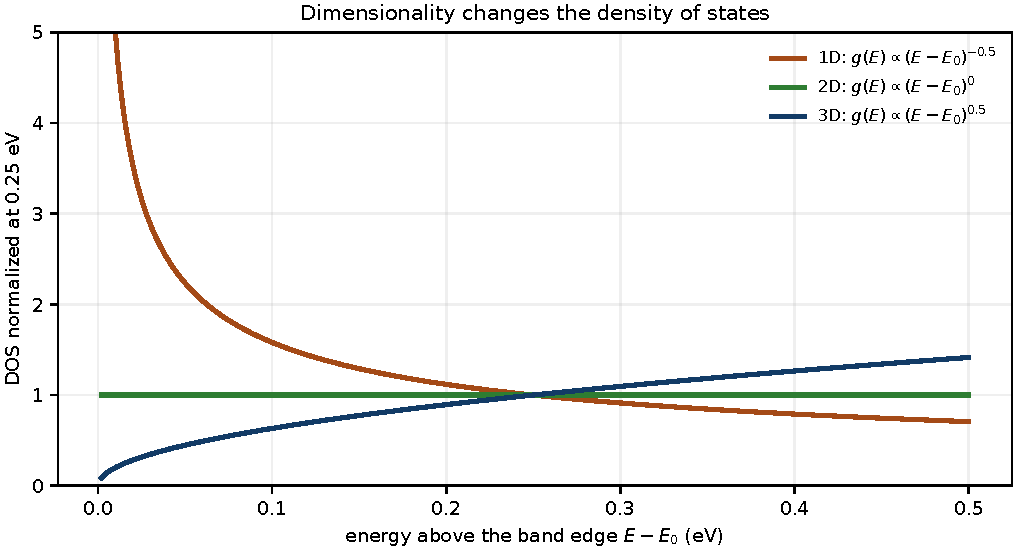
\includegraphics[width=0.78\textwidth]{figures/dos-dimensionality.pdf}
  \caption{The parabolic density of states depends qualitatively on spatial
  dimensionality.  Normalization at a common energy places the three shapes on
  one dimensionless scale.\figurenotebookmark}
  \label{fig:dos-dimensionality}
\end{figure}
\figurenotebooktext{figures/03_spectral-density-of-states/fig_03_02.ipynb}

\section{Anisotropic valleys and the density-of-states mass}

Near an anisotropic three-dimensional minimum, choose principal axes so that
\begin{equation}
  E(\bm q)
  =E_0+\frac{\hbar^2}{2}
   \left(
     \frac{q_1^2}{m_1}
    +\frac{q_2^2}{m_2}
    +\frac{q_3^2}{m_3}
   \right).
  \label{eq:dos-anisotropic-parabolic-band}
\end{equation}
The constant-energy surface is an ellipsoid with semiaxes
\begin{equation}
  q_i^{\max}
  =\frac{\sqrt{2m_i\varepsilon}}{\hbar}.
  \label{eq:dos-ellipsoid-semi-axes}
\end{equation}
Its reciprocal-space volume is
\begin{equation}
\begin{aligned}
  \Omega_k(\varepsilon)
  &=\frac{4\pi}{3}q_1^{\max}q_2^{\max}q_3^{\max}\\
  &=\frac{4\pi}{3}
    \left(\frac{2\varepsilon}{\hbar^2}\right)^{3/2}
    \sqrt{m_1m_2m_3}.
\end{aligned}
  \label{eq:dos-ellipsoid-volume}
\end{equation}
Define
\begin{equation}
  \boxed{
  m_d=(m_1m_2m_3)^{1/3}.
  }
  \label{eq:dos-effective-mass-definition}
\end{equation}
Then $m_d^{3/2}=\sqrt{m_1m_2m_3}$, so the anisotropic state count has the same
form as an isotropic calculation with mass $m_d$.

This replacement preserves the reciprocal-space volume enclosed by a constant-
energy surface.  Direction-dependent velocity and conductivity retain the full
effective-mass tensor.  The density-of-states mass governs state counting; the
transport mass governs directional response.

If there are $g_v$ equivalent valleys, their contributions add:
\begin{equation}
  g_c(E)
  =\frac{g_sg_v}{4\pi^2}
   \left(\frac{2m_d}{\hbar^2}\right)^{3/2}
   \sqrt{E-E_C}\,\Theta(E-E_C).
  \label{eq:multivalley-conduction-dos}
\end{equation}
A mass convention that incorporates $g_v$ already represents the complete
valley count.

\section{Several bands at the same energy}

The total density of states is additive:
\begin{equation}
  g(E)=\sum_n g_n(E).
  \label{eq:dos-band-additivity}
\end{equation}
For heavy- and light-hole parabolic bands sharing a valence-band maximum,
\begin{equation}
\begin{aligned}
  g_v(E)
  ={}&\frac{g_s}{4\pi^2}
  \left(\frac{2}{\hbar^2}\right)^{3/2}
  \left(m_{hh}^{3/2}+m_{lh}^{3/2}\right)
  \sqrt{E_V-E}.
\end{aligned}
  \label{eq:heavy-light-hole-dos-sum}
\end{equation}
It is convenient to define a combined mass $m_{v,d}$ by
\begin{equation}
  m_{v,d}^{3/2}=m_{hh}^{3/2}+m_{lh}^{3/2},
  \label{eq:combined-valence-dos-mass-power}
\end{equation}
or
\begin{equation}
  m_{v,d}
  =\left(m_{hh}^{3/2}+m_{lh}^{3/2}\right)^{2/3}.
  \label{eq:combined-valence-dos-mass}
\end{equation}
This combined mass is a compact representation of the additive state count of
two distinct physical bands.

\section{Calculating a density of states from sampled bands}

An analytic expression is rarely available for an entire realistic band
structure.  Suppose band energies have been calculated on wave vectors
$\bm k_j$ with normalized reciprocal-space weights $w_j$:
\begin{equation}
  \sum_jw_j=1.
  \label{eq:dos-normalized-k-weights}
\end{equation}
The discrete approximation to the DOS per primitive cell is
\begin{equation}
  g(E)
  \simeq\sum_n g_n\sum_jw_j
  \delta\!\left[E-E_n(\bm k_j)\right],
  \label{eq:sampled-band-dos-delta-sum}
\end{equation}
where $g_n$ is the degeneracy assigned to band $n$.

A finite sample of wave vectors produces delta peaks.  To display a continuous
curve, replace each delta distribution by a normalized kernel.  For a Gaussian,
\begin{equation}
  \delta_\sigma(E-E_j)
  =\frac{1}{\sigma\sqrt{2\pi}}
   \exp\left[-\frac{(E-E_j)^2}{2\sigma^2}\right].
  \label{eq:dos-gaussian-kernel}
\end{equation}
Because
\begin{equation}
  \int_{-\infty}^{\infty}
  \delta_\sigma(E-E_j)\,\dd E=1,
  \label{eq:dos-gaussian-normalization}
\end{equation}
the integrated state count is preserved when the energy window contains the
broadened tails.

The width $\sigma$ defines the numerical energy resolution.  A separate
scattering model is required to interpret a width as a physical lifetime.
Large $\sigma$ values smooth spectral features, while small values resolve the
discreteness of the sampled $\bm k$ mesh.  Convergence requires coordinated
refinement of reciprocal-space sampling and energy resolution.

\begin{figure}[H]
  \centering
  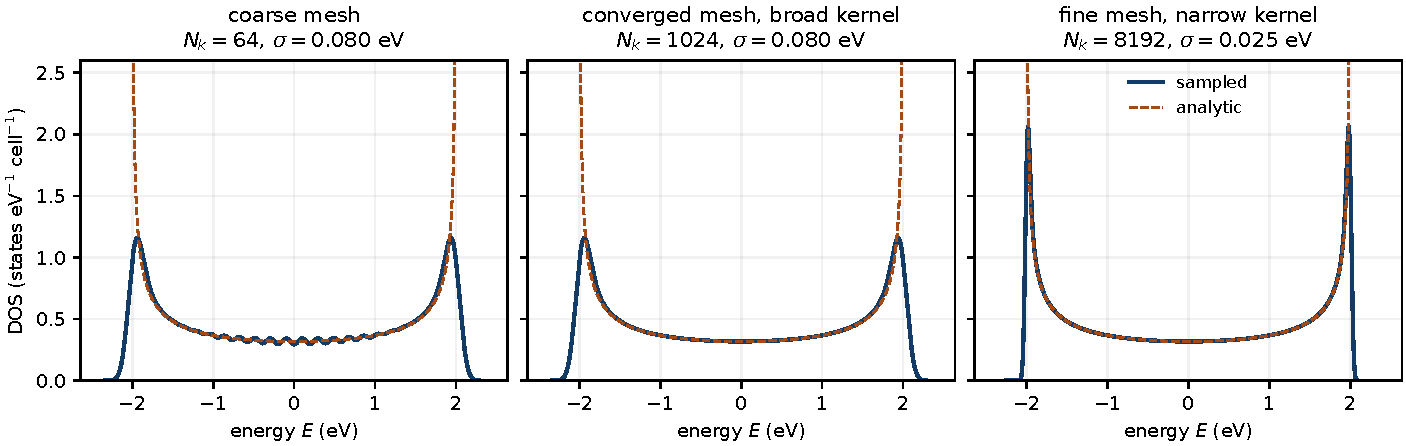
\includegraphics[width=0.98\textwidth]
    {figures/dos-numerical-convergence.pdf}
  \caption{Convergence of a DOS calculated from sampled tight-binding energies.
  A coarse reciprocal-space mesh produces visible sampling structure; excessive
  energy smoothing rounds the band-edge singularity; a fine mesh with a
  narrower normalized kernel approaches the analytic result.\figurenotebookmark}
  \label{fig:dos-numerical-convergence}
\end{figure}
\figurenotebooktext{figures/03_spectral-density-of-states/fig_03_03.ipynb}

An alternative is to partition energy into bins.  If bin $b$ has width
$\Delta E_b$, then
\begin{equation}
  g(E_b)
  \simeq\frac{1}{\Delta E_b}
  \sum_{n,j\,:\,E_n(\bm k_j)\in b}g_nw_j.
  \label{eq:dos-energy-bin-estimate}
\end{equation}
Division by bin width converts state counts into a density of states.  The
tetrahedron method in three dimensions instead uses local interpolation of the
bands to perform the Brillouin-zone integral.

\section{Normalization, units, and convergence}

Every DOS calculation should satisfy a state-count sum rule.  For a set of
complete bands represented per primitive cell,
\begin{equation}
  \boxed{
  \int_{-\infty}^{\infty}g(E)\,\dd E
  =\sum_n g_n.
  }
  \label{eq:dos-global-state-count-sum-rule}
\end{equation}
For a DOS per volume, the right side is divided by the primitive-cell volume.
A partial band or partial Brillouin-zone domain carries the corresponding
fractional state count.

A second check compares the integrated DOS
\begin{equation}
  \mathcal N(E)
  =\int_{-\infty}^{E}g(E')\,\dd E'
  \label{eq:integrated-density-of-states}
\end{equation}
with an independent count of states below $E$.  Unlike the DOS, which can be
singular or noisy, $\mathcal N(E)$ is monotonic and often reveals normalization
errors clearly.

A third check varies the physical and numerical resolution.  The wave-vector
mesh is refined together with the energy-bin or smoothing width, and the energy
interval is expanded until the normalization integral is stable.  The final
integral uses explicit energy and spatial units and counts every degeneracy once.

\section{Computational laboratory: bands, state counting, and DOS}

The three figure notebooks in
\begin{center}
  \texttt{figures/03\_spectral-density-of-states/}
\end{center}
are organized by physical relation.  The first constructs a sampled
one-dimensional band and verifies its integrated state count, the second
compares the dimensional band-edge power laws, and the third examines
reciprocal-space and energy resolution.  Each notebook presents its direct
NumPy calculation before calling the reusable implementation that writes the
published figure.

The reusable numerical expressions are collected in
\texttt{figures/src/semphy/density\_of\_states.py}, with figure recipes in the
same package and tests in \texttt{figures/tests/semphy/}.  Every numerical
result is compared with an analytic limit or a state-count sum rule.

\section{Chapter summary}

The density of states is the spectral trace
$\mathcal V_d^{-1}\operatorname{Tr}\delta(E-\hat H)$.  The trace counts the
multiplicity of each eigenspace.  Bloch's theorem resolves a periodic
Hamiltonian into bands, and periodic boundary conditions establish the
reciprocal-space state density.  The delta-function expression converts the
band map $E_n(\bm k)$ into an energy density, while its constant-energy-surface
form explains why slowly varying bands and critical points produce large or
singular contributions.  Parabolic bands give inverse-square-root, constant,
and square-root behavior in one, two, and three dimensions, respectively.
Anisotropy enters the three-dimensional state count through the geometric mean
of the principal masses.  For sampled bands, reciprocal-space weights, energy
resolution, degeneracy, normalization, and convergence must all be declared.
The next chapter applies statistical mechanics to determine the occupation of
these available states.
